%!TEX root = ../thesis.tex

\chapter{Preliminaries}
\label{chap:prelim}
\section{Classification} 
\label{sec:class}
\todo[line]{Maybe integrate these sections in chapter one} In this thesis we will mostly be concerned with qualitative learning, often called \textit{classification}, which is as follows. \todo{reference to Hatsie here?} We have a, usual finite, set of labels called $Y=\set{y_1,\ldots y_n}$ and for a given input $X$ we are expected to pick one of the labels to attach to it. Going back to our spam example this would look like $Y=\set{spam, genuine}$. As with this example it is useful to note that these labels usually lack any kind of structure like a order or magnitude, even though they are usually labelled with numbers. In the case that we have only two labels we will usually take them to be 1 and -1, so in our spam example labelling a email as genuine would get attached a 1 and spam a -1. 

\section{Boosting}
\label{sec:boost}
% \begin{wrapfigure}{r}{0.5\textwidth}
%   \begin{center}
%     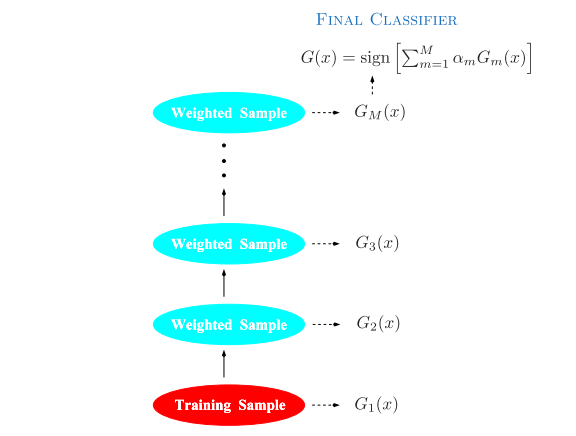
\includegraphics[width=0.48\textwidth]{images/boosting.png}
%   \end{center}
%   \caption{An illustration of the boosting process\cite{Hastie2009}}
%   \label{im:boost}
% \end{wrapfigure}   
% \todo{reproduce picture using my own notation}
Let us give a more detailed description of the process of boosting. Firstly we require a set of training data we will call $T$ and a weak \todo{should I introduce weaklearn again because maybe people haven't read the full introduction?}learning algorithm called \weak. The procedure is to fit \weak on our training data which produces a hypothesis $h_t:X\to Y$. When we receive the hypothesis we also receive a loss vector. This loss vector is a measure for how well we have done and is usually the error of \weak on the training set. Using this received loss vector we will slightly alter the training set by attaching weights to them, which measure their importance and then repeat the process. 